%
% File: chap01.tex
%
\let\textcircled=\pgftextcircled
\chapter{Introduction}
\label{chap:intro}

\initial{N}uclear power is coming to a turning point, which will likely decide its future. Second generation reactors designs, developed in the 50s and 60s, are used today to generate most of the world's nuclear energy. Accidents like Chernobyl and Fukushima have led to heavy criticism of the nuclear industry by a large number of lay people.

Several third generation reactor designs are being built today to replace the world aging nuclear fleet, but they are already under criticism, being considered too risky. The fourth generation reactor design developments are still underway, and have the ability to change lay people's view on this source of energy. This can be accomplished only if the risks are analyzed and taken into account to the best of our abilities, and if these studies' results are communicated efficiently to the unforgiving public opinion.

%=======
\section{A brief design introduction}
\label{sec1:design_intro}

\newacronym{sfr}{SFR}{Sodium-cooled Fast Reactor}

One of the designs currently under development is the \gls{sfr}. This is the most advanced fourth generation reactor design, and around twenty SFRs have already been operated throughout the world. First introduced by the USA in 1951 in Idaho Falls, Russia, France and Japan are today the main players, with India and China having also recently developed their prototypes. Two different designs exist for the SFR, pool-type (figure~\ref{fig:c1f1}, figure~\ref{fig:c1f2}) and loop-type (figure~\ref{fig:c1f2})~\cite{iaea01}. This study will focus on the pool-type design.


% A single figure
\begin{figure}[t!]
	\centering
	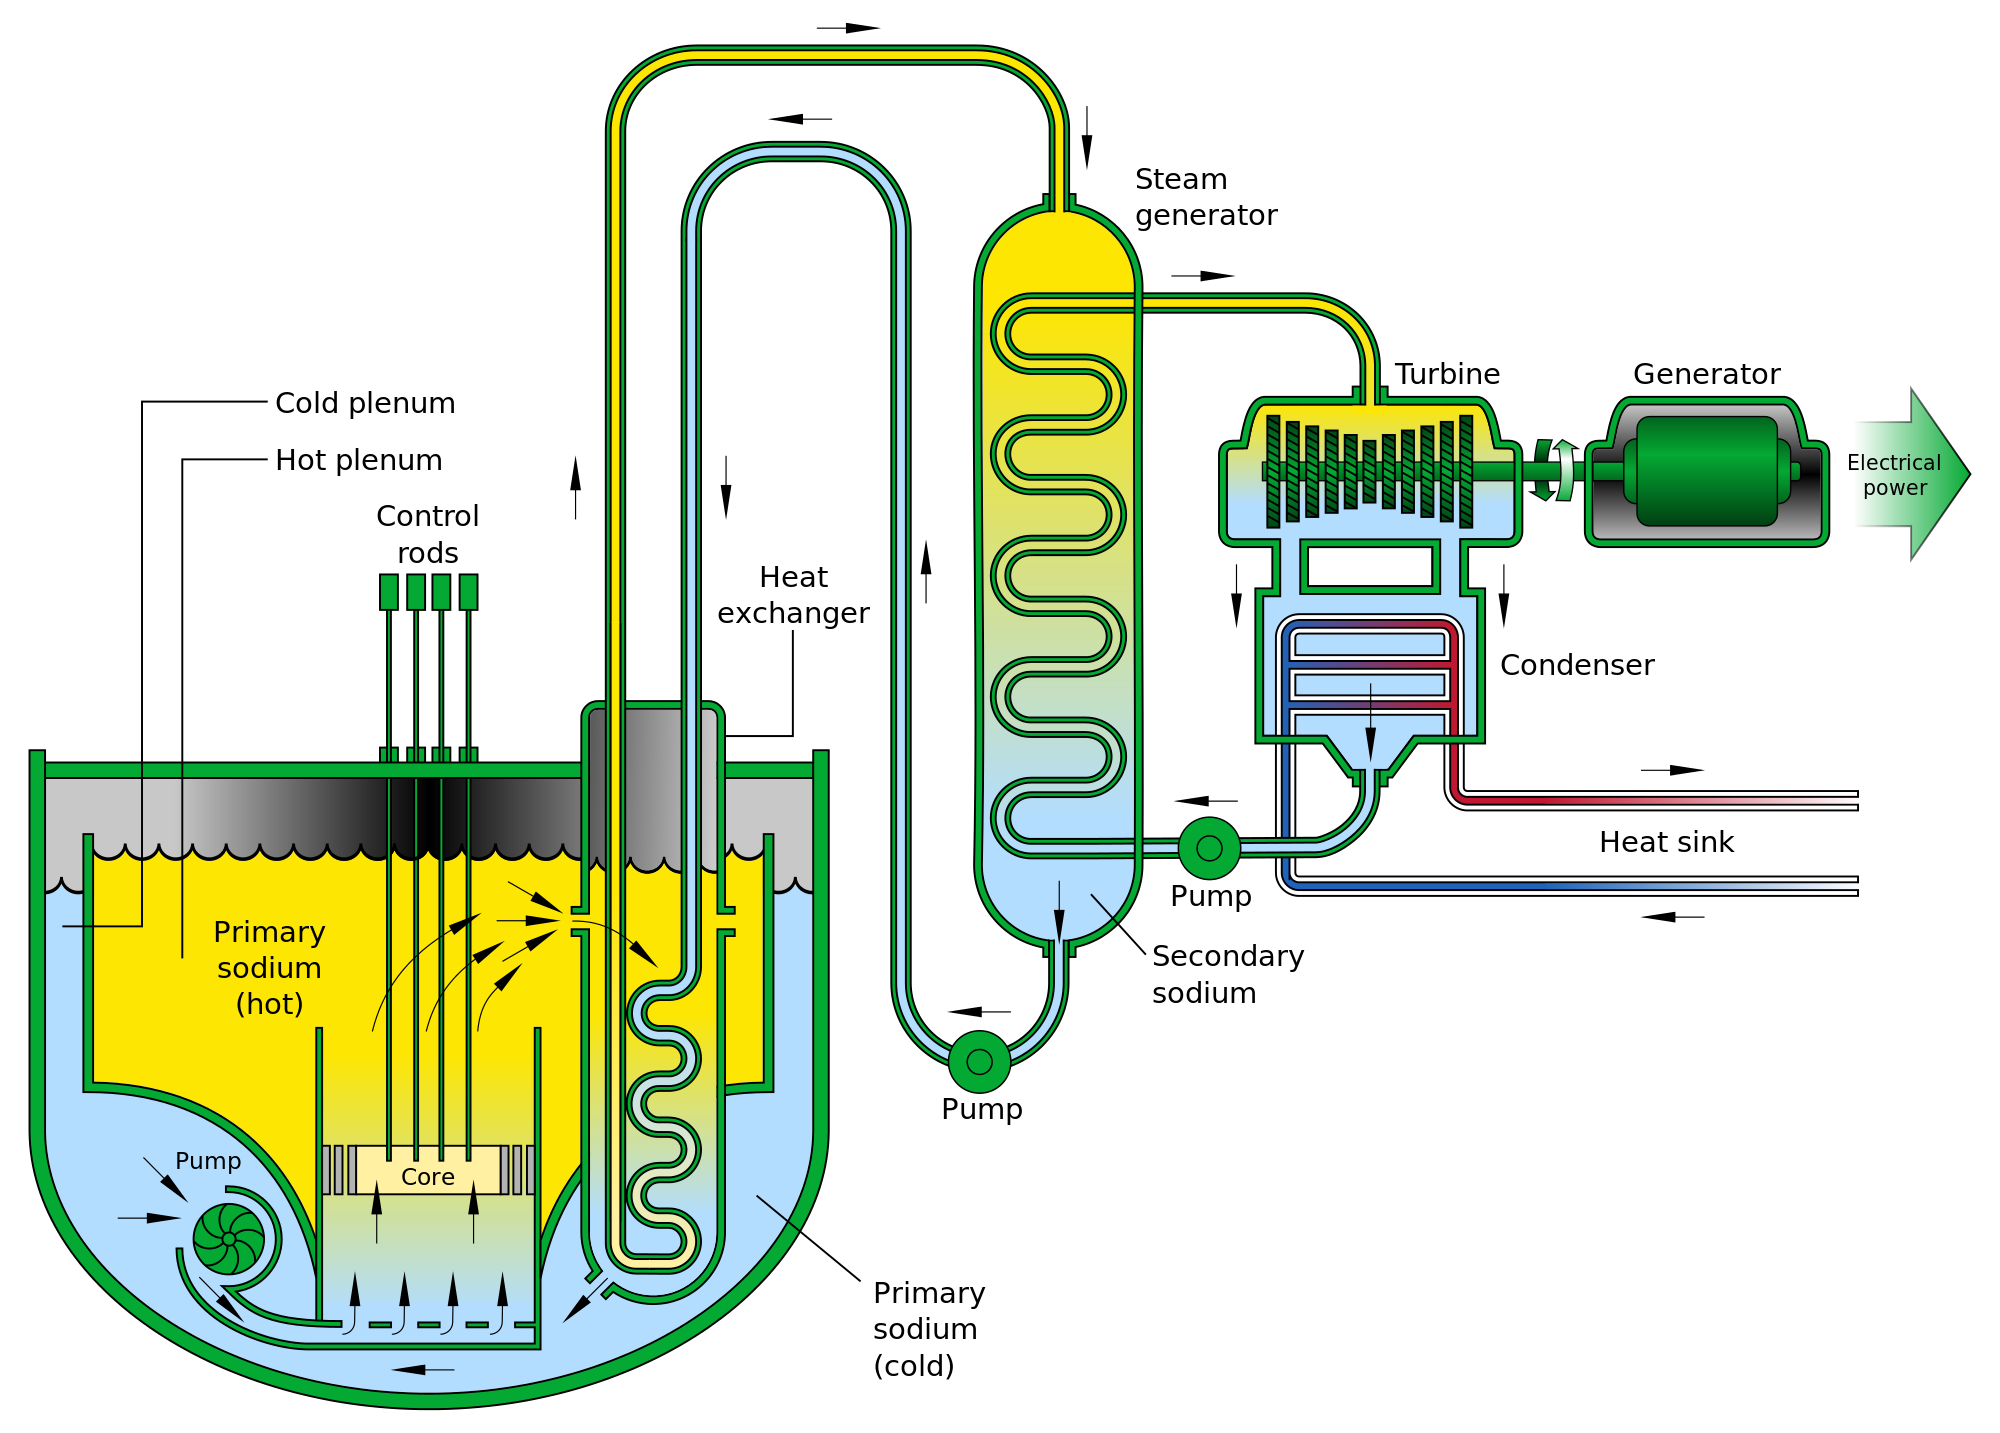
\includegraphics[height=0.5\textheight]{fig01/Sodium-Cooled_Fast_Reactor_Schemata}
	\mycaption[Pool type sodium-cooled fast reactor]{Pool type sodium-cooled fast reactor.}
	\label{fig:c1f1}
\end{figure}

\begin{figure}[t!]
	\centering
	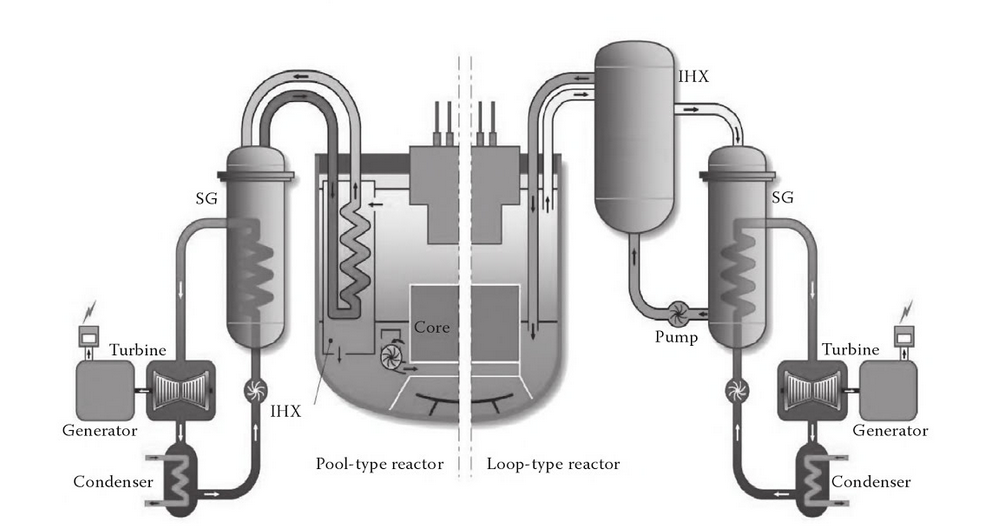
\includegraphics[height=0.4\textheight]{fig01/SFR_pool_loop_types}
	\mycaption[Pool-type vs Loop-type sodium-cooled fast reactor]{Pool-type vs Loop-type sodium-cooled fast reactor.}
	\label{fig:c1f2}
\end{figure}

Table~\ref{tab:c1t1} shows a simplified comparison of the pros and cons of this fourth generation design, not inherently specific to the SFR. Some advantages and inconvenients are found in other GEN IV designs.


\begin{table}[!htb]
    \begin{center}
        \begin{tabular}{ | l | p{5cm} | p{5cm} |}
        \hline
        Category & Pros & Cons \\ \hline
        \multirow{4}{*}{Technology} & Flexible fuel cycle (U, Pu, Th) & Opaqueness of Na \\
                                    & Breeding and Transmutation & Na reacts with air and water \\
                                    & Core power density & Shielding fast spectrum \\
                                    & High thermal efficiency & High operation temperatures \\ \hline
        \multirow{2}{*}{Economics} &  & Expensive R\&D \\
                                   &  & Expensive design \\ \hline
        Politics & & New set of regulations \\ \hline   
        Environment & Waste reduction &  \\ \hline
        Opinions & & Hostile public opinion \\
        \hline
        \end{tabular}
        \caption{Highly simplified advantages/inconvenients table for the SFR design}\label{tab:c1t1}
    \end{center}
\end{table}

%=======
\section{A bit of history}
\label{sec1:history}

Several SFR have been in operation in the world, accumulating around 400 reactor-years of feedback. Even though the technologies used in each reactor design is not identical, similarities are such that parallels can be drawn and applied to our case study design. Some of the reactors in this international feedback are loop-type, instead of the pool-type design considered in this study, but most incidents and repairs would be applicable to both designs.

The feedback from the different reactors show one recurrent failure, sodium leaks. Even though the consequence of this failure have not had catastrophic consequences, they could potentially be important. Notably, they will be one of the main point of interest during public debates. Failure modes causing sodium leak (loss of coolant, fire and explosion hazard), especially on a large scale, will thus be considered with attention.

\subsection{A focus on SUPERPHENIX}
\label{subsec1:superphenix}

The French Superhenix reactor demonstrates the impact of politics, public opinion and risk communication in the nuclear industry.

The reactor diverged in 1985 and was connected to the grid and reached full power in 1986, just as Chernobyl was happening. The worries that arose from the well-known accident caused an extremely violent opposition to the project. Several anti-nuclear organizations hence protested the project after Chernobyl, causing one death. It is to be noted that a rocket was even fired at the power plant.

\begin{figure}[t!]
	\centering
	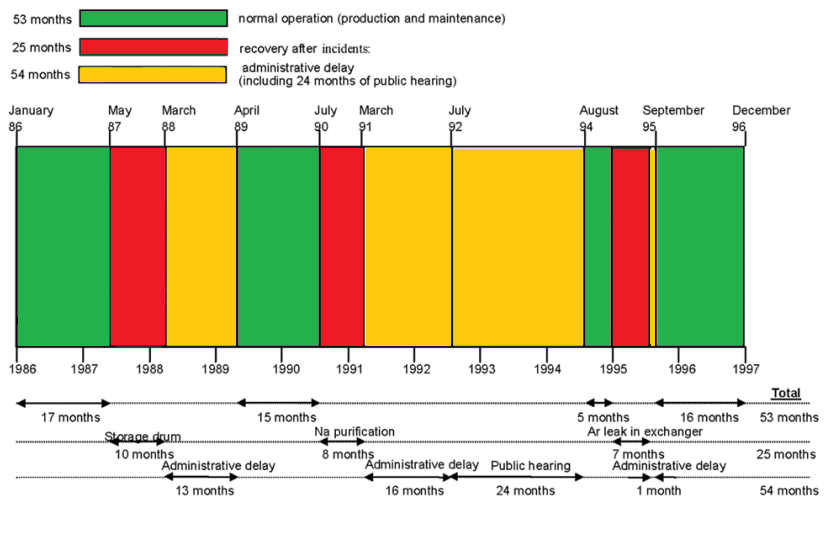
\includegraphics[height=0.35\textheight]{fig01/superphenix_timeline}
	\mycaption[Operation timeline for the SUPERPHENIX reactor]{Operation timeline for the SUPERPHENIX reactor~\cite{garcier01}.}
	\label{fig:c1f3}
\end{figure}

Consequently, due to growing concerns from the general public and political sides, the plant was shut down for extended periods of time not prominently for safety reasons, but mostly for administrative ones, and finally closed in 1997 following a political decision in an election period. In total, the plant was shut down 54 months due to purely administrative reasons~\cite{pris01}, when it would have been perfectly able to operate, over its 10 years operation (figure~\ref{fig:c1f3}).

This decision happened after the most productive year yet in the plant operation history, and caused a substantial loss, as the plant had to shut down in the middle of its cycle, wasting partially burnt up assemblies in the core and a whole new core refuel already assembled. The plant was supposed to stay online until at least 2015, and its early termination caused the operating company, EDF, to lose around roughly 4 billions dollars (lost fuel and partners reimbursement), on top of the lost revenues.

However, even though the decision to suddenly terminate the Superphenix project was mostly political, and driven by public opinion in the wake of Chernobyl, it would be wrong to consider that the technology used in this plant design was flawless and mastered, as obviously no system can be perfectly safe and reliable, and this was after all a prototype. The experts working on the project could not efficiently prove the system's safety to the (albeit ferociously opposed and potentially irrational) public. Failing such a crucial project in a "Nuclear country" could be a sign of an endangered industry going forward, a lack of communication skills from the experts, or a faulty design which could not be solidly defended.

\newacronym{astrid}{ASTRID}{Advanced Sodium Technological Reactor for Industrial Demonstration}

The shortfalls of Superphenix notably, and a few other SFR designs, will be used in this analysis to derive potential design flaws and communication problems and find some possible mitigations for the new French prototype \gls{astrid}, coming in the wake of yet another nuclear accident, Fukushima.


\subsection{International feedback}
\label{subsec1:feedback}


\subsubsection{American power plants}
\label{subsubsec1:usa}

After World War II, the USA were undeniably leaders in the nuclear industry, experimenting on a variety of audacious designs. They were the first to experiment with liquid-metal fast reactors, and in particular sodium-cooled reactors.

\textsc{Sodium Reactor Experiment} (1957-1964) was built to demonstrate the feasibility of a sodium-cooled reactor as the heat source for a commercial power reactor to produce electricity. It actually
experienced the first consequent meltdown of part of its (small) core in July 1959~\cite{ashley01}.

\textsc{Fermi-I} (1963-1972) was a 70MWe plant designed to test the feasability of breeding~\cite{fermi1}. It also suffered a partial meltdown in 1966, following a loss of coolant incident that was detected too late.

\newacronym{ebr}{EBR}{Experimental Breeder Reactor}

\textsc{EBR-I} (1951-1964) and \textsc{EBR-II} (1965-1994) were two \gls{ebr}, prototype of sodium-cooled fast reactors. EBR-II was one of the first reactors to exhibit passive safety systems that were tested and proven functional.

\subsubsection{French power plants}
\label{subsubsec1:france}

France has favored the Sodium-cooled fast reactors design in its history, following some american ideas and experiments.

\textsc{RAPSODIE} (1967-1983) was a pool-type prototype, the first of its kind built in France. Sodium aerosols were detected in the main vessel at some point, indicating a leak, which was not found. After the prototype was shut down, during the decommissioning, an explosion caused by an overpressure occurred in a sodium tank, killing one engineer and injuring four others.

\textsc{PHENIX} (1973-2010) followed in RAPSODIE footsteps. Several issues arose during the operation of this reactor. Those issues were identified and solved. They included numerous (32) sodium leaks and several (5) sodium-water reactions. In 2002, an explosion occurred in an almost empty sodium tank, due to water infiltrations after heavy rains. In 2008, an audit revealed important flaws in the plant anti-fire surveillance software.

\textsc{SUPERPHENIX} (1985-1997), discussed in greater details in~\ref{subsec1:superphenix}, also exhibited sodium leaks, including, in 1987, one near the safety vessel, due to steel-corrosion from an alloy not tested in its predecessors. Fixing this problem actually caused the loss of the fuel assemblies stockage ability, which penalized the subsequent plant operations. In 1990, the primary sodium got polluted, due to a defective membrane in a compressor. All in all though, the incidents in the primary circuit were scarce.

However, the plant underwent some more conventional troubles that impacted strongly the power generation. The machines room roof gave in after a snowstorm in 1990, and the initial design called for a 1200 MWe turbine, but the plant was finally equipped with two 600 MWe instead, impacting the plant grid availability.



\subsubsection{Russian power plants}
\label{subsubsec1:russia}

The reactors \textsc{BN-350} (1973-1999) and \textsc{BN-600} (1980-present) both experienced several sodium leaks, causing sodium fires for a couple hours. Not a lot of information is publicly available for those reactors.



\subsubsection{Japanese power plants}
\label{subsubsec1:japan}

Japan decided to go toward the loop-type design~ref{fig:c1f2}. \textsc{Joyo} was in operation for 30 years (1977-2007), and stopped its operations after an incident during fuel handling, preventing any subsequent core reload until removal of a bent subassembly.
On december 8, 1995, the secondary circuit of \textsc{Monju} (1986-present, but never in full operation) started vibrating, causing the leak of several hundreds kilograms of sodium. A fire happened with no automatic reactor shutdown. The reactor had to be shut down manually more than a hour later.


%=========================================================
